\chapter{Literatur}
Im Folgenden werden wichtige Begrifflichkeiten und Herleitungen, welche in dieser Arbeit verwendet werden, vorgestellt. Weitere theoretischen Grundlagen zu den vorgestellten Konzepten finden sich in den Arbeiten von \cite{Goodfellow-et-al-2016}, \cite{Kingma2014}.


\section{Few-Shot Learning}
Viele der heutigen \textit{State-of-the-Art} Modelle bauen auf einer riesigen Anzahl von Trainings Beispielen auf. Diese Anforderung kann aber nicht immer erfüllt werden. Bei nur wenig Beispielen ist daher die Gefahr des "Overfittings", d.h. des Auswendig Lernens des Datensatzes, entsprechend groß. Der Forschungsstrang "Few-Shot Learning" beschäftigt sich mit der Aufgabe, eine gute Generalisierung aus nur wenigen Daten zu Erzielen. Für $n$ Trainingsbeispiele pro $k$ Klassen spricht man von $n$-way $k$-shot Learning. \cite{Sung2017} erwähnen "Meta-Learning" als vielversprechenden Ansatz. Dieser geht, nach dem Paradigma "Lernen-zu-lernen" auf die Art zurück, wie Menschen lernen: Kinder haben kein Problem, aus einem einzelnen Bild das Objekt "Zebra" zu verstehen, da sie bereits das Konzept "Pferd" und "Farben" kennen. Kernidee in der von \cite{Sung2017} veröffentlichten Arbeit ist es eine Ähnlichkeitsfunktion zwischen Bildobjekten zu lernen. Realisiert wird dies durch Lernen eines Embedding-Vektors mit dem Ziel, dass ähnliche Objekte in diesem Raum nahe beieinander liegen. So können ungesehene Beispiele über einen "Nearest-Neighbor-Classifier" bekannten Beispielen zugeordnet und klassifiziert werden.

Ein alternativer Ansatz ist die Nutzung von Data Augmentation, um mehr Daten aus den vorhandenen zu erzeugen. Ein Vorteil dieses Weges besteht darin, dass für die Klassifikation wieder auf \textit{State-of-the-Art} Modelle zurückgegriffen werden kann. \cite{Antoniou2017} zeigen, dass auch Generative Modelle dazu verwendet werden können, um Data Augmentation zu betreiben. Mit Hilfe von vielen generierten Daten können gute Generalisierungen erzielt werden.



\section{Autoencoder}\label{sec:autoencoder}
Der Autoencoder (AE) stellt eine Encoder-Decoder Architektur dar (siehe Abb. \ref{fig:ae_model}. Aufgabe des Encoders $f$ ist es, die Eingabe $x$ in einen Merkmalsraum abzubilden. Anschließend versucht der Decoder $g$ die Eingabe zu rekonstruieren. Die Ausgabe des Autoencoders ist somit die Komposition $g(f(x))$. Um eine präzise Rekonstruktion zu erzielen, werden Fehlerfunktionen der folgenden Art verwendet:
\begin{equation}
  \cL(x, g(f(x)))
\end{equation}
Demnach können Autoencoder in einem selbst-überwachten Szenario trainiert werden. Übliche Fehlerfunktionen zur Bewertung der Diskrepanz zwischen $x$ und $g(f(x))$ sind "Binary-Cross-Entropy-Loss" und "Mean-Squared-Error". In Bezug auf die Dimension des Merkmalsraums unterscheidet man zwei Fälle. \\
\begin{figure}[hbt]
\centering
  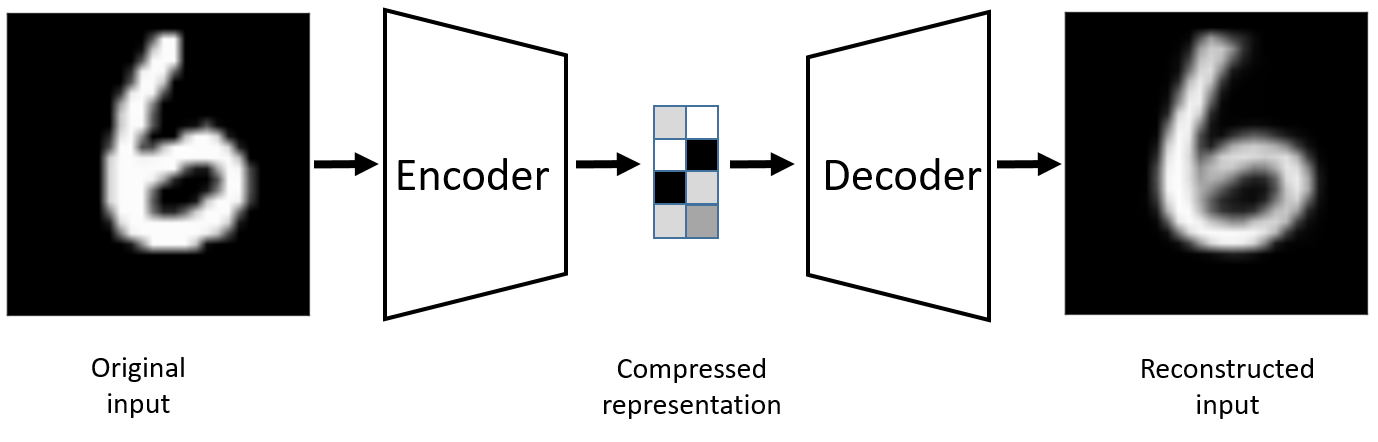
\includegraphics[width=.8\textwidth]{gfx/literature/autoencoder}
  \caption{Die Encoder-Decoder Struktur des "undercomplete" Autoencoders. Der Encoder berechnet eine komprimierte Repräsentation der Eingabe. Der Decoder ist in der Lage diese wieder zu einem Bild zu rekonstruieren. Abb. entnommen aus \cite{LopezPinaya2019}.}
  \label{fig:ae_model}
\end{figure}
Der erste Fall ist der sogenannte "undercomplete" AE. Hierbei wird die Dimension des Merkmalsraums kleiner als die der Eingabe gewählt, sodass dieser einen Flaschenhals für den Informationsfluss bildet. Der Encoder komprimiert die Eingabe und stellt so eine Dimensionsreduktion dar. Falls der Autoencoder $(f \circ g)$ durch eine lineare Abbildung definiert ist, entspricht diese Dimensionsreduktion einer "Principle-Component-Analysis" (PCA) (siehe \cite{ladjal2019pcalike}). Eine Definition über nicht-lineare Abbildungen ist deutlich mächtiger. An dieser Stelle bieten sich Neuronale Netze an, da sie beliebige, insbesondere nicht-lineare Funktionen, approximieren können. Zudem sind (Konvolutionale-) Neurale-Netzwerke (CNN) eine weit verbreitete Methode der automatisierten Merkmalsextraktion. Ein üblicher Nutzen von "undercomplete" Autoencodern ist eben dieser komprimierte Merkmalsvektor als Repräsentant der Eingabe.\\
Der zweite Fall ist der "overcomplete" Autoencoder. Anders als zuvor wird hier die Dimension des Merkmalsraums größer als die der Eingabe gewählt. Dadurch bildet der Encoder keinen Flaschenhals und ist folglich auch nicht gezwungen, Merkmale zu extrahieren. Der "overcomplete" Autoencoder lernt den Datensatz auswendig ("Overfitting"). Dies führt zum Strukturverlust im Merkmalsraum. Um diesem Verhalten entgegen zu wirken, werden Regularisierungstechniken angewandt. Eine dieser Regularisierungen, Denoising Autoencoder, wird im Folgenden vorgestellt. Weitere Regularisierungstechniken sind z.B. "Sparse-Autoencoder", "Contractive-Autoencoder" und "Conditional-Autoencoder" (nachzulesen in \cite{LopezPinaya2019}). Man bemerke, dass diese Varianten auch bei "undercomplete" Autoencodern zu einem stabileren Training beitragen können.

\begin{figure}[hbt]
  \centering
  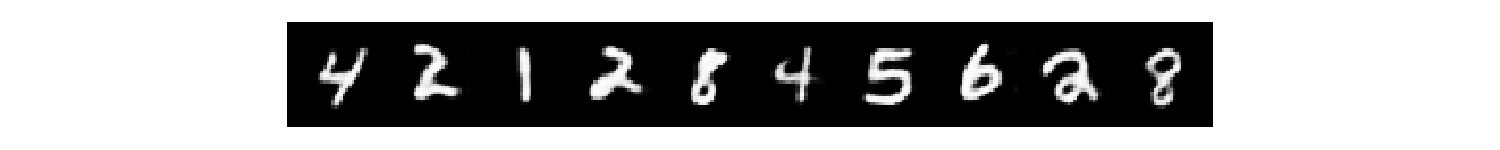
\includegraphics[width=\textwidth]{gfx/literature/reals}
  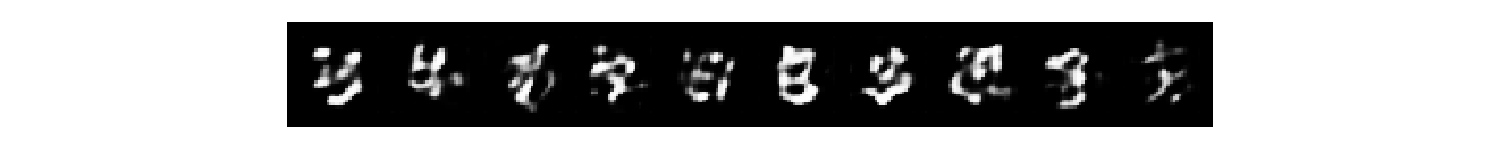
\includegraphics[width=\textwidth]{gfx/literature/fakes}
  \caption{Zwei Rekonstruktionen von Vektoren aus dem Feature Space. Die Beispiele oben sind ein codierte Eingaben, welche anschließend decodiert wurden. Unten dargestellt sind zufällige decodierte Merkmalsvektoren.}
  \label{fig:ae_reconstruction}
\end{figure}


\subsection{Denoising Autoencoder}\label{sec:dae}
Der Denoising Autoencoder (DAE) betrachtet statt der Eingabe $x$ ein modifiziertes $\tilde{x}$. Die Modifikation wird durch Addition von Rauschen z.B. aus einer uniformen oder einer Normalverteilung erreicht. Diese Regularisierungstechnik führt offensichtlich dazu, dass der DAE robust gegenüber Rauschen in den Eingabebildern wird. Außerdem erfolgt eine bessere Exploration des Merkmalsraumes. DAEs verwenden Fehlerfunktionen der folgenden Art:
\begin{equation}\label{eq:DAE}
  \cL(x, g(f(\tilde{x})))
\end{equation}

\begin{figure}[hbt]
  \centering
  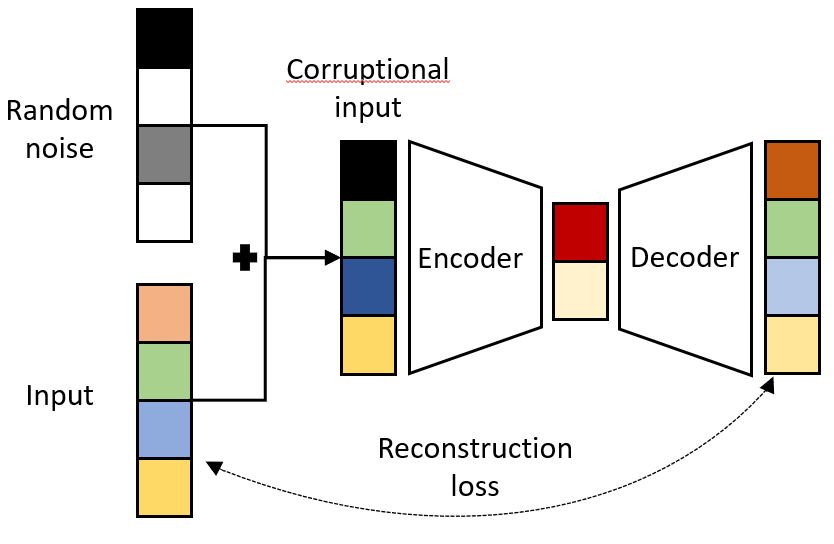
\includegraphics[width=.6\textwidth]{gfx/literature/dae}
  \caption{Der DAE minimiert den Fehler zwischen der Rekonstruktion des modifizierten Eingabevektors und der Eingabe. Abbildung entnommen aus \cite{LopezPinaya2019}}
\end{figure}

Abb. \ref{fig:ae_reconstruction} zeigt zwei Rekonstruktionen von Merkmalsvektoren. Man beachte, dass ein zufälliges Sample aus dem Merkmalsraum mehr einem Rauschen als einer tatsächlichen Klasse aus dem Datensatz ähnelt. Denn die Räume zwischen den codierten Merkmalsvektoren sind im Allgemeinen nicht definiert. Der Merkmalsraum besitzt keine "geometrische" Struktur. Um dieses Problem zu lösen wurde eine weitere Klasse von Autoencodern entworfen: Variational Autoencoder.



\section{Variational Autoencoder}\label{sec:VAE_introduction}\label{sec:variational_autoencoder}
\cite{Kingma2014} betrachten in ihrer Arbeit das Konzept des Autoencoders aus einer probabilistischen Sicht. Der Encoder bildet die Eingabe nicht auf einen eindeutigen Merkmalsvektor, sondern auf eine Wahrscheinlichkeitsverteilung über den Merkmalsraum ab. Damit bekommt der Merkmalsraum eine probabilistische Struktur. Die Herleitung des Variational Autoencoders erfolgt üblicherweise über das Konzept von latenten Variablen, welches im Folgenden näher erläutert wird. Die Herleitung Orientiert sich an den Arbeiten von \cite{Kingma2014} und \cite{Doersch2016}.


\subsection{Latente Variablen}
Latente Variablen sind nicht beobachtbare Zufallsvariablen (ZV), welche aber aus einem mathematischen Model heraus gefolgert werden können. Eine Latente Variable kann zum Beispiel eine codierte Merkmalsbeschreibung eines Bildobjektes sein. Diese gibt vor wie das Objekt aussieht, tatsächlich beobachtet werden, kann aber nur das Objekt selbst. Den Zufallsraum der latenten Variable wird Latent-Space genannt.\\
In den anschließenden Kapiteln werden die folgenden Bezeichnungen verwendet:
\begin{itemize}
  \item $\cD$, der Datensatz über einen Raum $\cX$, respektive $x \sim D$, mit $x \in X$ ein beliebiger Datenpunkt aus dem Datensatz.
  \item $\cZ = \bR^d$, der Latent-Space mit Dimension $d$
  \item $P\left[ \cZ\right]$ eine "probability density function" (PDF) über $\cZ$.
  \item $\mu_\phi: \cX \rightarrow \cZ$, eine beliebige Funktion parametrisiert durch $\phi$. Wird im folgenden verwendet, um den Erwartungswert einer Normalverteilung $\cN$ zu approximieren.
  \item $\sigma_\phi: \cX \rightarrow \cZ$, analog zu $\mu_\phi$, die Varianz der Normalverteilung $\cN$.
  \item $g_\theta: \cZ \rightarrow \cX$, beliebige Funktion parametrisiert durch $\Theta$. Repräsentiert den Decoder.
\end{itemize}
$\mu_\phi(x)$ und $\sigma_\phi(x)$ repräsentieren gemeinsam die Ausgabe des Encoders für Eingabe $x$.\\

Sei die PDF $P\left[ \cZ \right]$ beliebig aber fest. Außerdem sei $z \in Z$ eine Latente Variable, mit $z \sim P\left[ \cZ\right]$. Für ausreichend komplexe $g_\theta$ kann durch die Wahl von $\Theta$ jede beliebige Verteilung mittels $g_\theta$ modelliert werden (Inverse-Transform-Sampling). Sei nun $P_\theta(x \vert z) = P\left(g_\theta(z) = x \right)$ die bedingte Wahrscheinlichkeit des Auftretens von $x$. Über Marginalisierung erhalten wir:
\begin{equation}\label{eq:max_likelihood}
  P_\theta(x) = \bE_{z \sim P(\cZ)} \left[ P(x \vert z) \right] = \int_{\cZ} P_\theta(x \vert z) \cdot P(z) dz
\end{equation}
Um den Datensatz möglichst gut zu repräsentieren, soll $P_\theta\left[ \cX \right]$ nach der "Maximum-Likelihood" Methode maximiert werden. Dazu sind folgende Ableitungen nötig:
\begin{equation}
  \frac{\partial}{\partial \theta} P_\theta(x) = \int_{\cZ} \frac{\partial}{\partial \theta}P_\theta(x \vert z) \cdot P(z) dz
\end{equation}
Dieses Integral ist im Allgemeinen nicht lösbar. Dennoch kann es approximiert werden. Eine Möglichkeit dies zu tun ist Monte-Carlo-Integration. Dieser Ansatz ist allerdings nicht effizient, denn $\cZ$ ist überabzählbar. Erweiterungen der Monte-Carlo Integration (z.B. "Importance Sampling") sind auch nicht anwendbar, da keine Annahmen über die Verteilung $P_\theta(x \vert z)$ möglich sind. Bekannt ist aber, dass $P_\theta(z \vert x)$ die bedingte Wahrscheinlichkeit darstellt, dass $z$ im Urbild (bzgl. $g_\phi$) von $x$ liegt, sprich $z$ ist Erzeuger von $x$. Ziel ist es, $P_\theta(z \vert x)$ zu approximieren, um gezielt die $z$ zu sampeln, welche $x$ erzeugen. Gesucht ist also eine Verteilung $Q\left[ \cZ \right]$, welche ähnlich zu $P_\theta\left[ \cZ \vert x\right]$ ist. Dazu wird im anschließenden Abschnitt die Kullback-Leibler Divergenz eingeführt.


\subsection{Kullback-Leibler Divergenz}
Die Kullback-Leibler Divergenz, kurz KL Divergenz oder $\cD_{KL}$, ist ein Maß für die Ähnlichkeit zweier Wahrscheinlichkeitsverteilungen. Für beliebige Verteilungen $Q, P$ über eine Menge $\cX$ ist sie definiert als:
\begin{equation}
  \cD_{KL}\left[ Q \| P\right] = \bE_{x \sim Q}\left[ \log Q(x) - \log P(x)\right]
\end{equation}
Mit der KL Divergenz und dem Satz von Bayes kann die Beziehung zwischen $P(x)$ und $\bE_{z \sim Q}\left[ P(x \vert z )\right]$ formuliert werden:
\begin{align}
  \cD_{KL}\left[ Q\left[ \cZ \right] \| P_\theta\left[ \cZ \vert x\right] \right] &= \bE_{z \sim Q}\left[ \log Q(z) - \log P_\theta(z \vert x)\right] \\
  &= \bE_{z \sim Q}\left[ \log Q(z) - \log(\frac{P_\theta(x \vert z) \cdot P(z)}{P_\theta(x)})\right] \notag\\
  &= \bE_{z \sim Q}\left[ \log Q(z) - \log P_\theta(x \vert z) - \log P_\theta(z) + \log P_\theta(x)\right] \notag
\end{align}
Da $\log P_\theta(x)$ nicht von $z$ abhängt kann dieser Term aus dem Erwartungswert gezogen werden.
\begin{equation}
  \cD_{KL}\left[ Q(z) \| P_\theta(z \vert x)\right] = \bE_{z \sim Q}\left[ \log Q(z) - \log P_\theta(x \vert z) - \log P(z)\right] + \log P_\theta(x) \notag
\end{equation}
Dies ist äquivalent zu:
\begin{align}
  \underbrace{\log P_\theta(x)}_\text{Log-Likelihood} - \underbrace{\cD_{KL}\left[ Q\left[ \cZ \right] \| P_\theta\left[ \cZ \vert x\right] \right]}_\text{Error Term} &= - \bE_{z \sim Q}\left[ \log Q(z) - \log P_\theta(x \vert z) - \log P(z)\right] \notag\\
  &= \bE_{z \sim Q}\left[ \log(P_\theta(x \vert z)\right] - \cD_{KL}\left[ Q(z) \| P(z)\right] \label{eq:pre_objective}
\end{align}
Zu sehen ist auf der linken Seite dieser Gleichung zunächst die logarithmierte Wahrscheinlichkeit von $x$ (Log-Likelihood), welche maximiert werden soll. Von dieser wird die KL-Divergenz von $Q$ und $P$ subtrahiert. D.h. $P_\theta(x)$ wird maximiert und gleichzeitig $Q\left[ \cZ \right]$ dafür bestraft, zu weit von der tatsächlich unterliegenden Verteilung $P_\theta\left[ \cZ \vert x\right]$ abzuweichen. Die rechte Seite besteht aus dem Erwartungswert von $z \sim Q$ über folgende Terme: Die Log-likelihood $g_\phi(z) = x$ und die KL-Divergenz von $Q(z)$ und $P(z)$. Man beachte, dass $g_\phi(z)$ berechnet werden kann und $P\left[ \cZ \right]$ beliebig ist. Es wird nun $P\left[ \cZ \right]$ und $Q$ spezifiziert. Üblicherweise wird $P\left[ \cZ \right]$ als $\cN(0, I)$ gewählt ($I \in \bR^{d \times d}$ ist die Einheitsmatrix) . $Q\left[ \cZ \right]$ wird parametrisiert durch $Q_\phi\left[ \cZ \vert x \right] = \cN(\mu_\phi(x), \sigma_\phi(x))$. $\sigma_\phi(x)$ ist die Hauptdiagonale der Kovarianzmatrix $\Sigma_\phi(x)$. Eine Annahme für VAEs ist nähmlich, dass die Dimensionen in $\cZ$ unkorreliert sind und folglich $\Sigma_\phi$ diagonal ist. Vorteil dieser Parametrisierung von $Q$ ist, dass sich die Ableitung der KL-Divergenz von Normalverteilungen effizient berechnen lässt. Einsetzen in \ref{eq:pre_objective} ergibt:
\begin{align}\label{eq:objective}
  &\log P_\theta(x) - \cD_{KL}\left[ Q\left[ \cZ \right] \| P_\theta\left[ \cZ \vert x\right] \right] \notag\\[8pt]
  =& \, \bE_{z \sim \cN(\mu_\phi(x), \sigma_\phi(x))}\left[ \log \underbrace{P_\theta(x \vert z)}_\text{Decoder} - \cD_{KL}[\underbrace{\cN(\mu_\phi(x), \sigma_\phi(x))}_\text{Encoder} \| \cN(0, I)] \right]
\end{align}
Gleichung \ref{eq:objective} zeigt direkt die Encoder-Decoder Struktur der VAE Zielfunktion.
\begin{figure}[hbt]
  \centering
  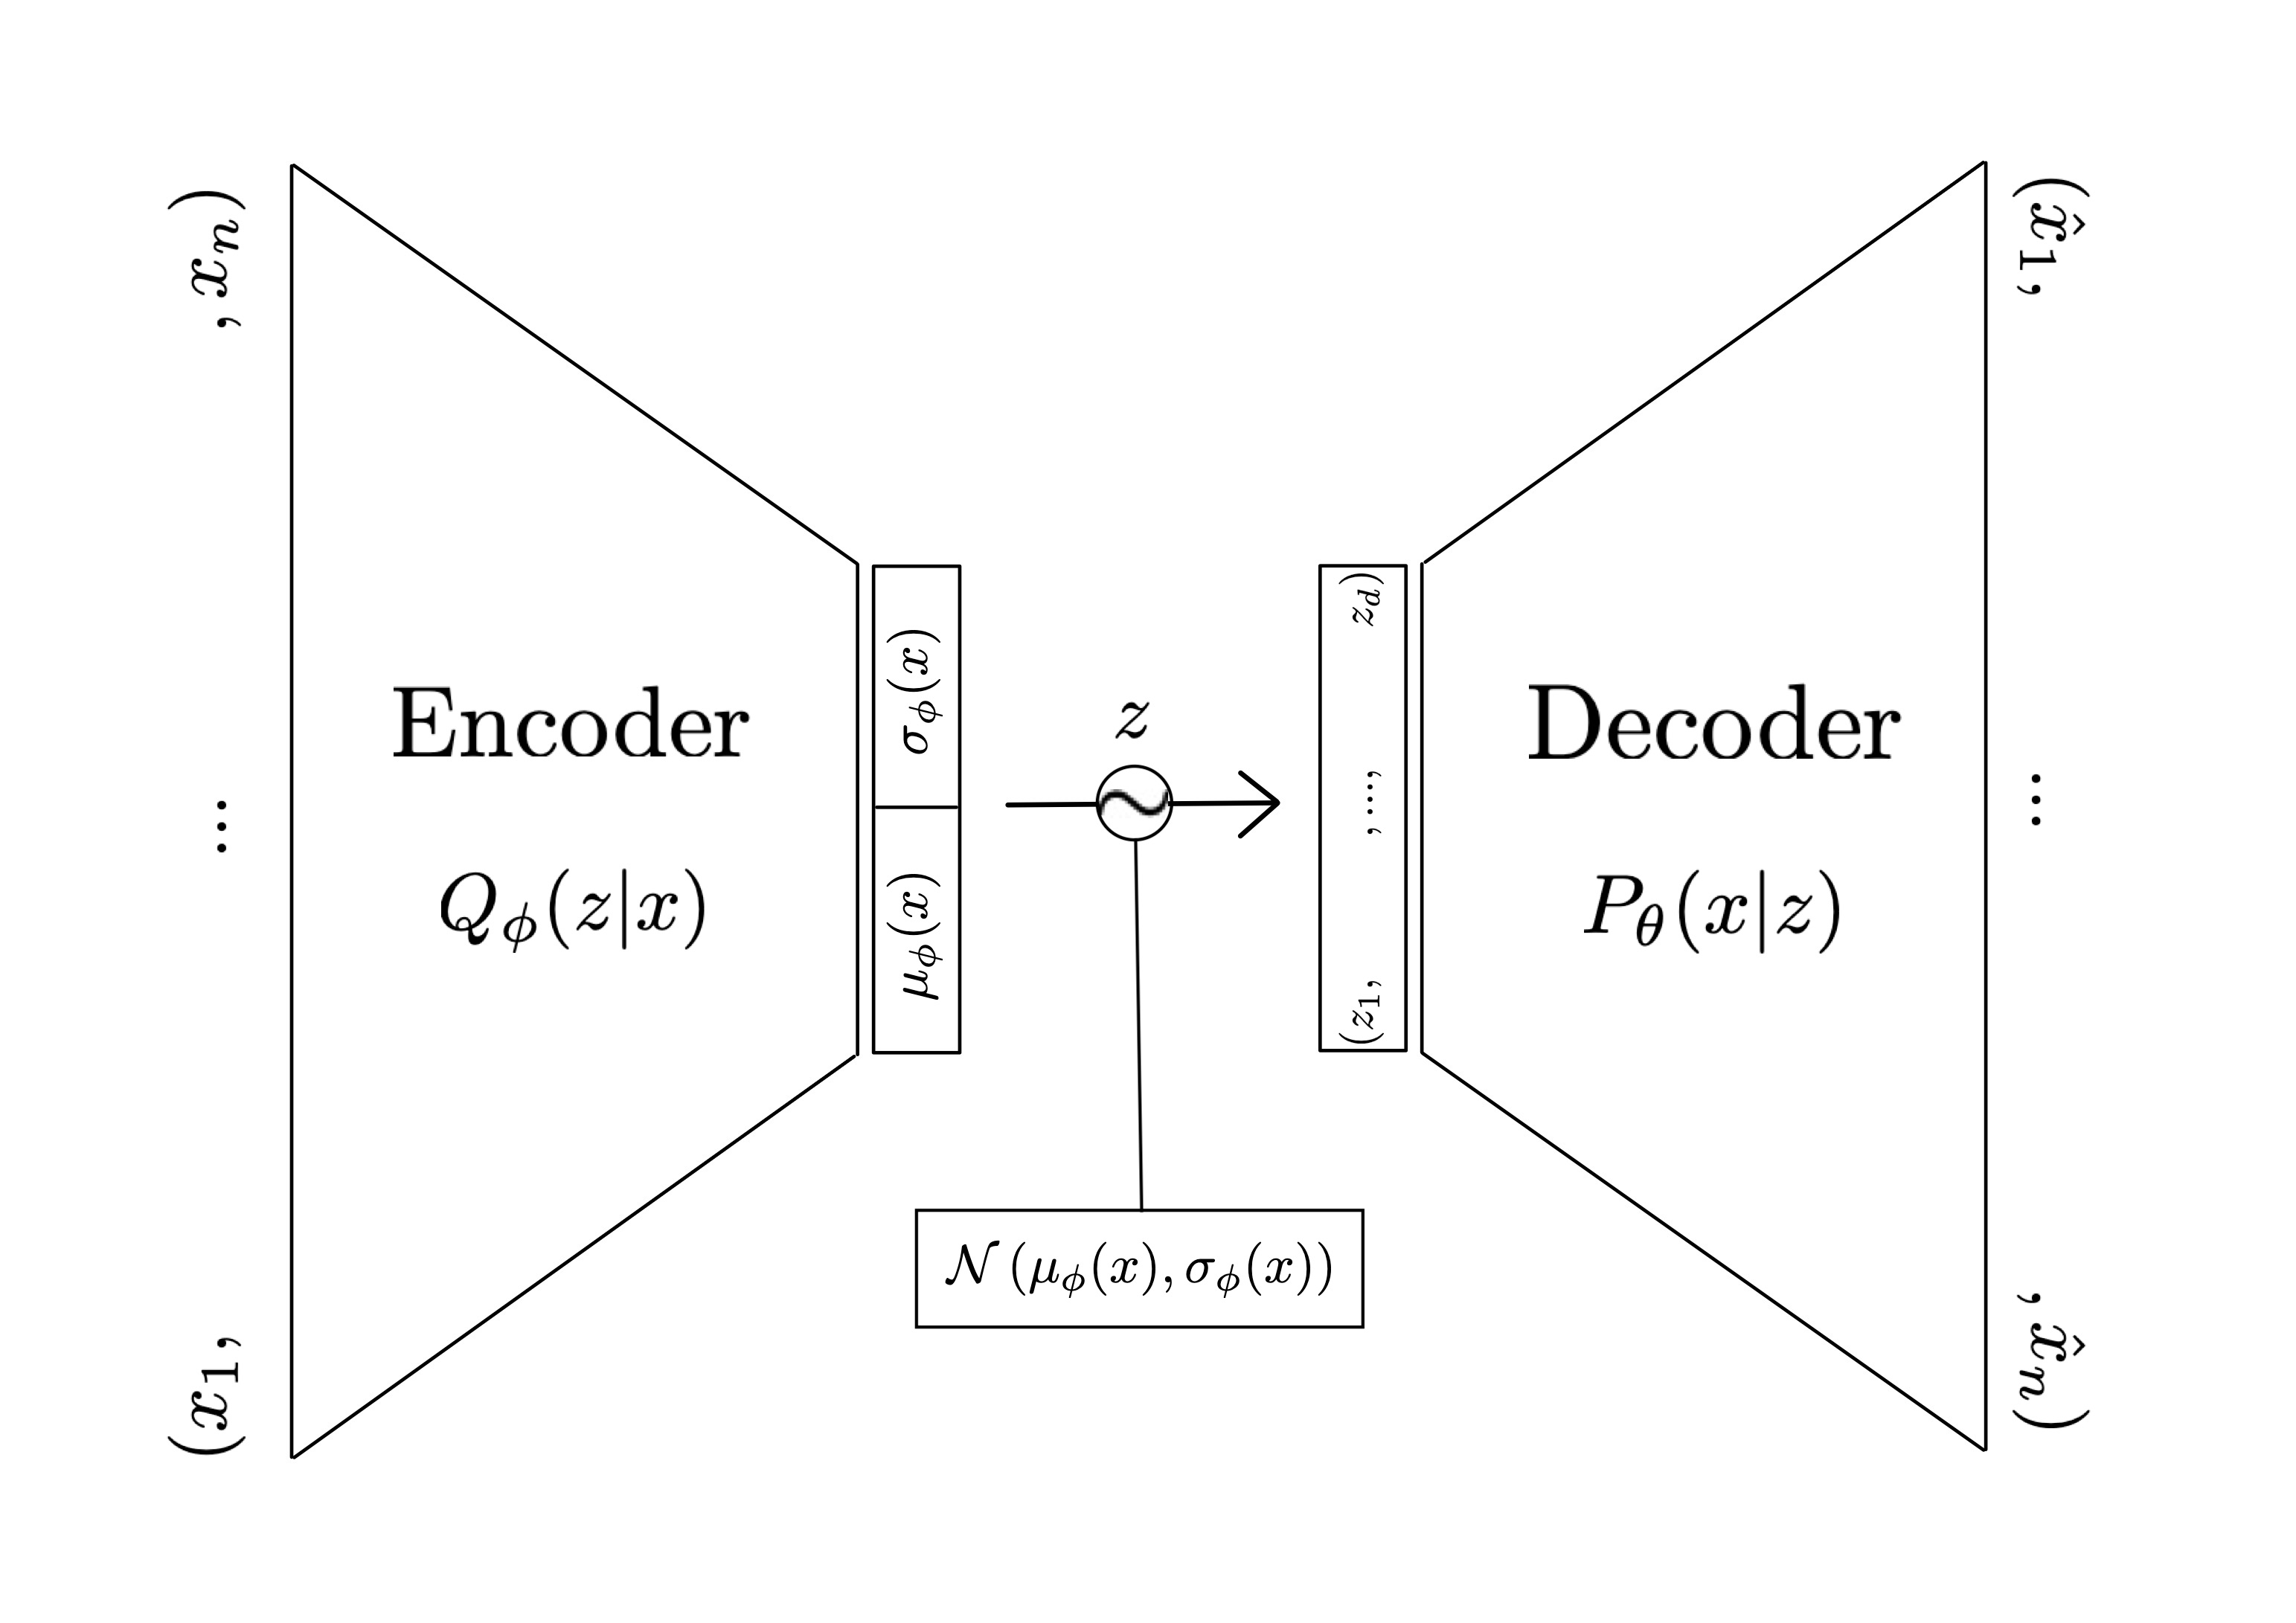
\includegraphics[width=.7\textwidth]{gfx/literature/forward_pass}
  \caption{Der Vorwärtsdurchlauf beim VAE. Der Encoder die Verteilung $Q_\phi(z \vert x)$ parametrisiert durch $\mu_\phi$ und $\sigma_\phi$. Aus dieser wird $z$ erzeugt. Anschließend liefert der Decoder die Rekonstruktionsverteilung $P_\theta(x \vert z)$ bzw. für festes $x$ die Rekonstruktion $\hat{x}$. (siehe auch \cite{Doersch2016}}
  \label{fig:enc-dec}
\end{figure}


\subsection{Optimierung der VAE Zielfunktion}\label{sec:vae_loss_func}
Statt die obige Zielfunktion zu maximieren, wird folgende Fehlerfunktion minimiert (der Einfachheit wegen wird $\mu_\phi$ statt $\mu_\phi(x)$ etc. geschrieben):
\begin{align}\label{eq:gradient}
  &\cL = - \left( \bE_{z \sim \cN(\mu_\phi, \sigma_\phi)}\left[ \log(P_\theta(x \vert z) - \cD_{KL}[\cN(\mu_\phi, \sigma_\phi) \| \cN(0, I)] \right] \right) \\
=& \, -\bE_{z \sim \cN(\mu_\phi, \sigma_\phi)}\left[ \log(P_\theta(x \vert z) \right] + \bE_{z \sim \cN(\mu_\phi, \sigma_\phi)}\left[ \cD_{KL}[\cN(\mu_\phi, \sigma_\phi) \| \cN(0, I)] \right]
\end{align}
Der erste Term entspricht dem komponentenweisen "Negative-Log-Likelihood" (NLL) Fehler der Eingabe $x$ und der Rekonstruktion $g_\theta(z)$. $z$ wird aus der Encoder Verteilung $\cN(\mu_\phi, \sigma_\phi)$ gesampelt. Für die KL Divergenz zweier Normalverteilungen existiert eine geschlossene Form zur Berechnung (siehe \cite{kl_divergence_close_form}):
\begin{align}
  &\cD_{KL}\left[ \cN(\mu_0, \Sigma_0) \| \cN(\mu_1, \Sigma_1)\right] = \notag\\
  &\frac{1}{2}\left( \Spur(\Sigma_1^{-1}\Sigma_0) + (\mu_1 - \mu_0)^T\Sigma_1^{-1}(\mu_1 - \mu_0) - k + \log(\frac{\det\Sigma_1}{\det\Sigma_0})\right)
\end{align}
Durch Einsetzen von $\cN(\mu_\phi, \sigma_\phi)$ und $\cN(0, I)$ vereinfacht sich die Gleichung zu:
\begin{align}
  &\cD_{KL}\left[ \cN(\mu_\phi, \Sigma_\phi) \| \cN(0, I)\right] = \notag\\
  &= \frac{1}{2}\left( \sum_{i=1}^k (\sigma_\phi)_i + \sum_{i=1}^k (\mu_\phi)_i^2 - \sum_{i=1}^k 1 - \log(\prod_{i=1}^k (\sigma_\phi)_i)) \right) \notag\\
  &= \frac{1}{2} \sum_{i=1}^k\left((\sigma_\phi)_i + (\mu_\phi)_i^2 - 1 - \log (\sigma_\phi)_i \right)
\end{align}
Die Ableitung des KL-Terms ist somit berechenbar. Für die Ableitung des NLL Fehlers nach dem Parametern $\phi$ des Encoders besteht jedoch folgendes Problem:
\begin{equation}
  \frac{\partial}{\partial \phi} (- \bE_{z \sim \cN(\mu_\phi, \sigma_\phi)}\left[ \log g_\theta(z) \right] )
\end{equation}
Da $z$ aus einer Zufallsverteilung gesampelt wird, kann keine Ableitung nach $\phi$ gebildet werden. Als Lösung wird der folgende Trick angewandt.

\subsection{Reparametrisierungs-Trick}\label{sec:reparam_trick}
Eine Ableitung des NLL Fehlers ist nach den Parametern $\phi$ des Encoder Netzwerks wegen des Samplings von $z \sim \cN(\mu_\phi, \sigma_\phi)$ nicht möglich. Statt aber direkt aus der Verteilung zu sampeln, kann ein $\epsilon \sim \cN(0, I)$ gesampelt werden und die gleiche Verteilung durch Multiplikation und Addition berechnet werden. Für $z \sim \cN(\mu_\phi(x), \sigma_\phi(x))$ gilt also:
\begin{equation}
  z = (\sigma_\phi(x))^{\frac{1}{2}} \cdot \epsilon + \mu_\phi(x)
\end{equation}
D.h. von folgender Gleichung kann die Ableitung nach $\phi$ berechnet werden:
\begin{equation}
  \frac{\partial}{\partial \phi} \left(- \bE_{x \sim D}\left[ -\bE_{\epsilon \sim \cN(0, I)}\left[ \log g_\theta\left(z = (\sigma_\phi(x))^{\frac{1}{2}} \cdot \epsilon + \mu_\phi(x)\right)\right] \right] \right)
\end{equation}
